%# -*- coding: utf-8-unix -*-
% !TEX program = xelatex
% !TEX root = ../thesis.tex
% !TEX encoding = UTF-8 Unicode

\section{关系理解:知识库补全任务}
\label{sec:rw-kbc}

%Part 1: 什么是KBC

现有的知识库具包含了庞大数量的实体和事实,但其中的内容仍然不够完全,
尤其是存在大量的长尾实体,并没有多少事实与之相关。
因此,知识库补全任务(Knowledge Base Completion, KBC)的目的,
是向已有知识库中添加缺失的事实三元组($e_1$, $p$, $e_2$)。
这些新增的三元组中,无论是谓词$p$还是它的两个参数实体$e_1$和$e_2$,
都已存在于知识库中。
换言之,新增的事实并不会给知识库带来额外的节点,或是从没见过的边,
而是让知识库的图结构更加稠密。

新增事实三元组(尤其是参数实体)的获取方式通常有两种。
第一种来源为经过了实体链接过后的外部文本,纯文本或表格文本均可称为来源。
%
对于纯文本,当在句中定位两个参数实体后,
句子剩下的部分成为了描述实体间关系的上下文。
此时即可依据上下文信息来预测对应的知识库谓词,
即等价于关系分类问题,相关研究包括词级别卷积神经网络\cite{xu2015semantic}
以及依存语法路径上循环神经网络\cite{xu2015classifying}。
对于表格文本,知识库补全关注于表格的两列之间,利用表列所包含的实体,
判断两列之间的关系是否与知识库中特定谓词对应,实现可能的大批量事实补全。
例如\figref{fig:rw-linking-limaye},
Title和Author列之间的关系被映射到YAGO中的$Writes$谓词。
%主要使用的方法有
%如概述中指出,  表格关系可以补充三元组
%Munoz:找关系 挖掘不同行之间,但是是同样的两列之间的实体关系,映射至DBPedia 构成三元组,即挖掘语义。  并补充缺失
%在维基百科内部(已有链接)
%按已有match比例尝试一些predicate,然后学习一个triple是对还是错
%Sekhavat: Tabular KBC 同样是假设linking已好的情况 利用PATTY作为跳板,根据EP之间存在的pattern,寻找到rel的关系
%条件概率  (相当于EP有一系列的外部文本pattern,而不是仅有KB)
%rel来自YAGO
%(Fuck...但两者根本都是column-column-rel和predicate的一一对应)

第二种来源不涉及到任何知识库外的信息,新增三元组来自于知识库的内部挖掘,
通过寻找不同谓词之间的关联,推理出可能缺失的事实。
例如\secref{sec:intro-background}提到的例子,
``{某人的国籍缺失,可以根据其出生地所在的国家进行推测}'' ,
人类可以通过这样的方式进行知识的手动补充,正是因为掌握了
国籍、出生地、地点被包含这三个谓词之间的关联。
这条路线不受知识库外信息的干扰,因此是我们关注的研究点。

学术界已有工作在此场景上研究知识库补全的解决方案,
并提出了相关的KBC数据集,
例如FB15k\cite{bordes2013translating}和WN18\cite{bordes2014semantic},
分别是Freebase和WordNet的子集。
对于知识库补全模型的测评,主要通过
主宾语预测(Link Prediction)以及三元组分类(Triple Classification)
这两个子任务来进行。
前者为三元组($e_1$, $p$, $?$)或($?$, $p$, $e_2$)预测缺失的主语或宾语,
后者则判断给定的($e_1$, $p$, $e_2$)是否为正确事实。
两者虽然形式不同,但都需要计算三元组的置信分:$S(e_1, p, e_2; KB)$。

解决知识库补全的方法主要分为两类。
第一类基于规则推导,用逻辑表达式描述实体间存在特定谓词时,所需要满足的特定规则;
第二类基于知识库向量,学习所有实体、谓词的连续特征表示,
并挖掘三元组各部分特征表示之间存在的深层代数关系。
下面将分别介绍这两种方法。

\subsection{基于规则推导的模型} %基于规则推导的关系语义推理模型

基于规则推导的模型旨在使用人类可以直接理解的规则形式,来描述不同谓词之间的联系,
即如果$e_1$和$e_2$之间满足特定的条件,则推理出三元组($e_1$, $p$, $e_2$)成立。
为方便论述,我们将三元组以布尔表达式$p(e_1, e_2)$表示,
若对应三元组存在于知识库中,则表达式为真,否则表达式为假。
文献\parencite{lao2011random}以一个简单的推导规则为例:
若已知某运动员为球队效力,以及球队所处联盟,则可以推导出运动员所参与的体育联盟。
该规则可以通过一阶逻辑表达式进行形式化描述:
\begin{equation}
\begin{aligned}
\exists b \in E, athletePlaysForTeam(a, b) & \land teamPlaysInLeague(b, c) \\
                                           & \implies athletePlaysInLeague(a, c),
\end{aligned}
\end{equation}
\noindent
其中$E$表示知识库实体集合。规则的左侧部分,使用的两个谓词实现了主语$a$到宾语$c$的连接,
且不包含多余的布尔表达式,因此这条规则表现为由谓词序列构成的路径。
对于``{依靠出生地推测国籍}'' 的规则,我们可以形式化为以下逻辑表达式:
\begin{equation}
\begin{aligned}
  \exists b \in E, placeOfBirth(a, b) & \land containedBy(b, c) \\
                                      & \land isA(c, country) \implies nationality(a, c),
\end{aligned}
\end{equation}
\noindent
其中谓词序列$\{placeOfBirth, containedBy\}$为连接主宾语的路径,
而谓词$isA$使得宾语$c$还需要满足额外的限制条件,因此这条规则具有比路径更加复杂的结构。

利用单个推导规则进行知识库补全存在两个局限:
首先,规则本身不一定完全正确,限制条件过于宽泛的规则可能打来错误的事实;
其次,单个规则的覆盖率较低,能够补全的知识有限。
针对这两个局限,已有的规则推导工作都致力于从知识库中挖掘目标谓词的多条规则,
并学习不同规则的重要性,以实现更健壮的知识库补全。

Lao等人提出的PRA模型\cite{lao2010fast}实现了规则的挖掘和学习。
对于目标谓词$p$,模型首先利用谓词已有的三元组($e_1$, $p$, $e_2$)作为训练数据,
在知识库中寻找所有能连通$e_1$和$e_2$的谓词序列,形成了多种路径形式规则。
模型利用逻辑回归实现规则权重的训练,以及对新三元组($e'_1$, $p$, $e'_2$)是否为真的预测。
每一条挖掘的规则类比为一个特征,对应的特征值为路径随机游走概率,
即从主语$e'_1$出发,沿规则的谓词序列随意跳转,最后到达$e'_2$的概率。
由于知识库中的谓词可能代表一对多关系,
因此随机游走概率值会小于1,甚至为0(无法通过当前规则连通)。
基于此,PRA模型能够快速抽取大量路径规则,并利用已知三元组在规则上随机游走概率实现权重训练。

一些研究工作对PRA模型进行了扩展。
文献\parencite{lao2011random}对挖掘的路径规则进行了限制,
要求规则至少要适用于训练数据中一定比例的主语,并对计算随机游走概率的采样方式进行了优化,
这两个扩展都是基于模型性能优化为考量。
%lao2011random
%改进1: 限制每条路径规则所能  满足的主语个数  以及连通的 训练三元组个数,  大幅度缩小规则数量
%改进2:随机游走的采样方式进行了优化。
Gardner等人提出了SFE模型\cite{gardner2015efficient},它在PRA模型基础上进行了两项改进:
首先,模型将作为特征值的随机游走概率替换为0/1特征,即只关心是否连通,
在大幅度提升运行速度的同时,对结果没有显著影响;
其次,模型引入不同于路径规则的其它特征,例如提取路径中的谓词bigram,
或由主语出发却不指向宾语的单边特征等,扩充特征集合以提升知识库补全效果。
%gardner2015efficient
%改进1:特征值转换为0/1对结果没有显著影响,PRA的具体概率值并不比0/1提供了更多信息(很惊讶),而PRA概率计算花费了大量时间
%改进2:引入了更多的规则,单边  anyrel, path bigram   并非基于路径的规则 but useful
Wang等人提出了CPRA模型\cite{wang2016knowledge},主要针对具有相似谓词的规则推导优化。
该模型通过层次聚类识别出具有相似语义的知识库谓词集合,
然后对每个集合内的谓词采用多任务学习框架,共享挖掘的规则特征和部分耦合参数,
使模型能够捕捉相似谓词之间的共性,实现隐式的训练数据共享。
%wang2016knowledge
%针对具有相似语义的知识库谓词,对它们的关系推理 过程   不独立,而是 能 彼此利用训练数据  互相影响,
%提出了  CPRA模型,   通过层次cluster识别  相似语义 的知识库谓词 ,   多任务学习 等方式 学习,
%使得  不同谓词的规则推导 不完全独立,   可以利用其它 的训练数据  优化自身。

%TODO: AMIE+, Zhang的放在内部related work说,有点太细了
% AMIE+
% 
% Zhang等人的研究 是 此任务 较早的工作。
% 文中称Ontological Smoothing, 为 特定关系寻找更多seed pair,
% 并用于relation extraction中,以提高pattern的准确率。
% 虽并不称作kbc,但本质相同。
% 提出了基于MLN的模型。
% 不仅
% 对每个谓词生成的规则由长度不超过4的谓词序列
% 同时对NELL 中的e和t都映射
% 
% 使用MLN学习每个规则的权重
% 对每个 谓词 相关规则   都寻找  合适的表达式,   谓词序列  考虑 并集
% 
% (类似的文章还有SQL query generation,见他的RW)
% 
% Zhang,MLN。。。
% %说各自的弱点
%   title={Learning to refine an automatically extracted knowledge base using markov logic},
%     goal: 过滤NELL,在candidate facts里寻找正确的fact。
%     rules: 好像并没有直接去学习p和p之间的关联,而是和meta predicate在搞?
%     model: MLN
%     
%   title={Large-scale knowledge graph identification using psl},
%     goal: 同上
%     rules: extractor, ontological, isA, relation
%     model: PSL, weight on rule, and also on the atom expression (KALE)
% 
%   title={Statistical schema induction},
%     太长了,先忽略
% 
% 
% 然后就终结在这里。不要再多了,ball ball u.

\subsection{基于知识库向量的模型}

与词向量模型类似,知识库向量的模型旨在学习一个知识库中的实体、谓词等元素
在连续空间的特征表达,以完成一系列下游任务。
具体在知识库补全任务中,
三元组置信分的计算并不依赖自动挖掘的推导规则,
而是来自主谓宾三者的连续特征表达在不同维度上的交互。
词向量模型依靠大规模的纯文本语料,
构建上下文单词预测任务来完成训练\cite{mikolov2013exploiting},
相比之下,知识库向量模型的训练过程更为直观:
利用知识库已有三元组作为训练数据正样本,
并自动生成不存在的三元组作为负样本,计算三元组置信分进行训练,
而这也恰好与知识库补全任务的目标一致。

知识库向量模型的优点在于所有谓词共同训练,更有效地利用训练数据,
并且能在连续空间中体现不同谓词的相似性,
但相应地,其缺点在于可解释性较弱。
不同的知识库向量模型对实体和谓词的特征表示具有不同的形式,
特征交互的方式也不尽相同,下面主要介绍几个具有代表性的模型。
%一类以RESCAL为代表,多层网络输出multi-layer perc;一类以TransE为代表,latent distance model

%类比词向量的训练,CBOW 等 依据上下文进行预测,相似语义 相似上下文
%类似的思路,信息来自已有的事实三元组,相似的实体 会有相似的谓词和另一个实体
%对于谓词也有类似的性质
%然而,上下文信息由三元组表示,准备好了更加准确的训练数据。
%以及实体和谓词并不是同一类东西,不能像word2vec那样,实体和谓词会在不同的空间中。
%From: A review of relational machine learning for knowledge graphs


\begin{figure}[htp]
  \centering
  \subcaptionbox{RESCAL模型\label{fig:rw-kbe:a}}
    {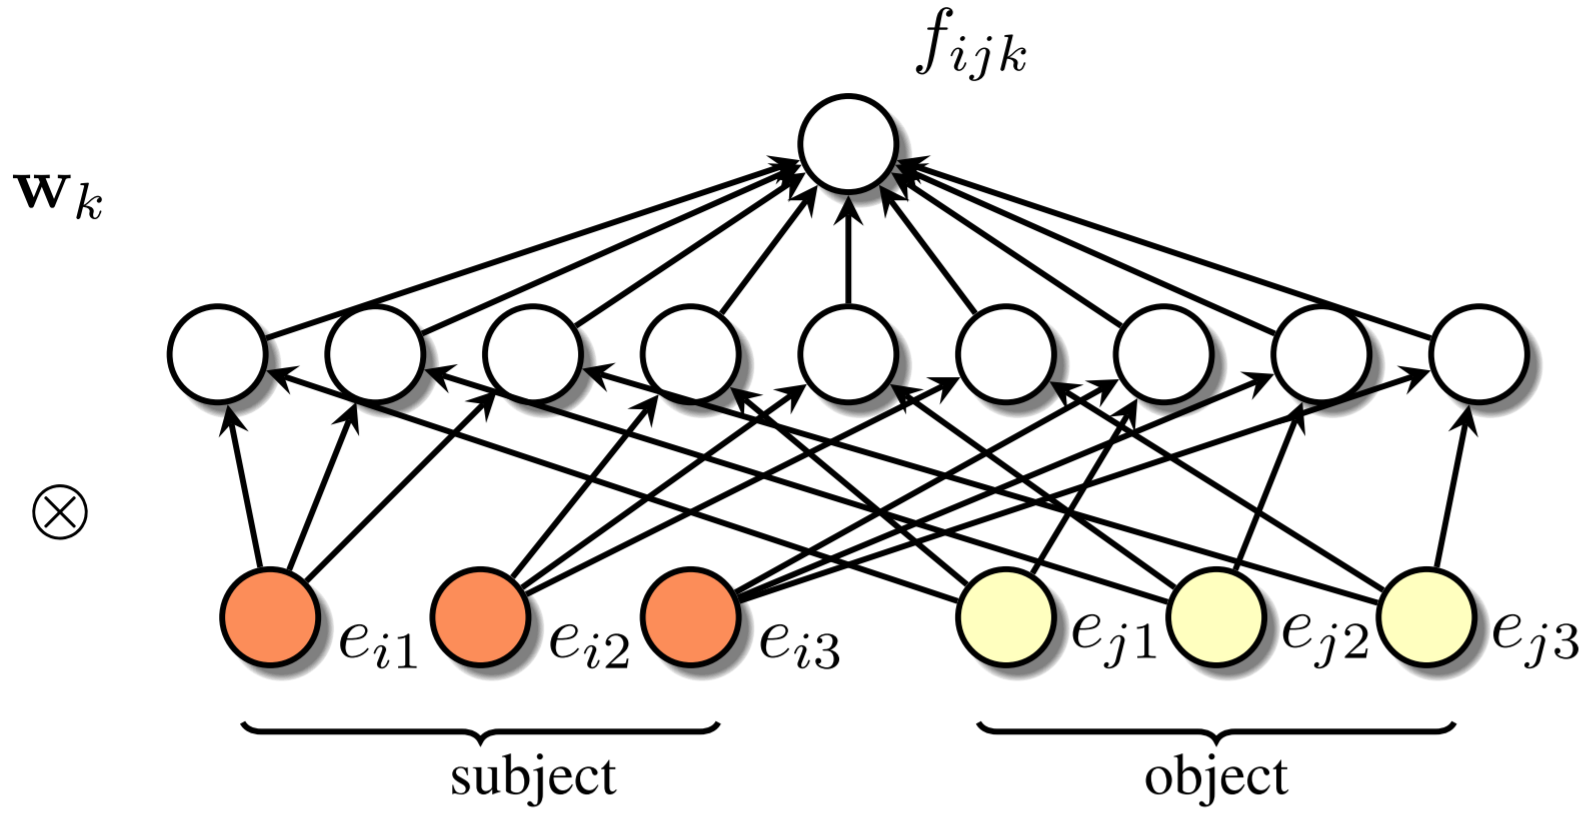
\includegraphics[width=0.48\columnwidth]{figure/rw/kbc-rescal.png}}
  \hspace{1em}
  \subcaptionbox{ER-MLP模型\label{fig:rw-kbe:b}}
    {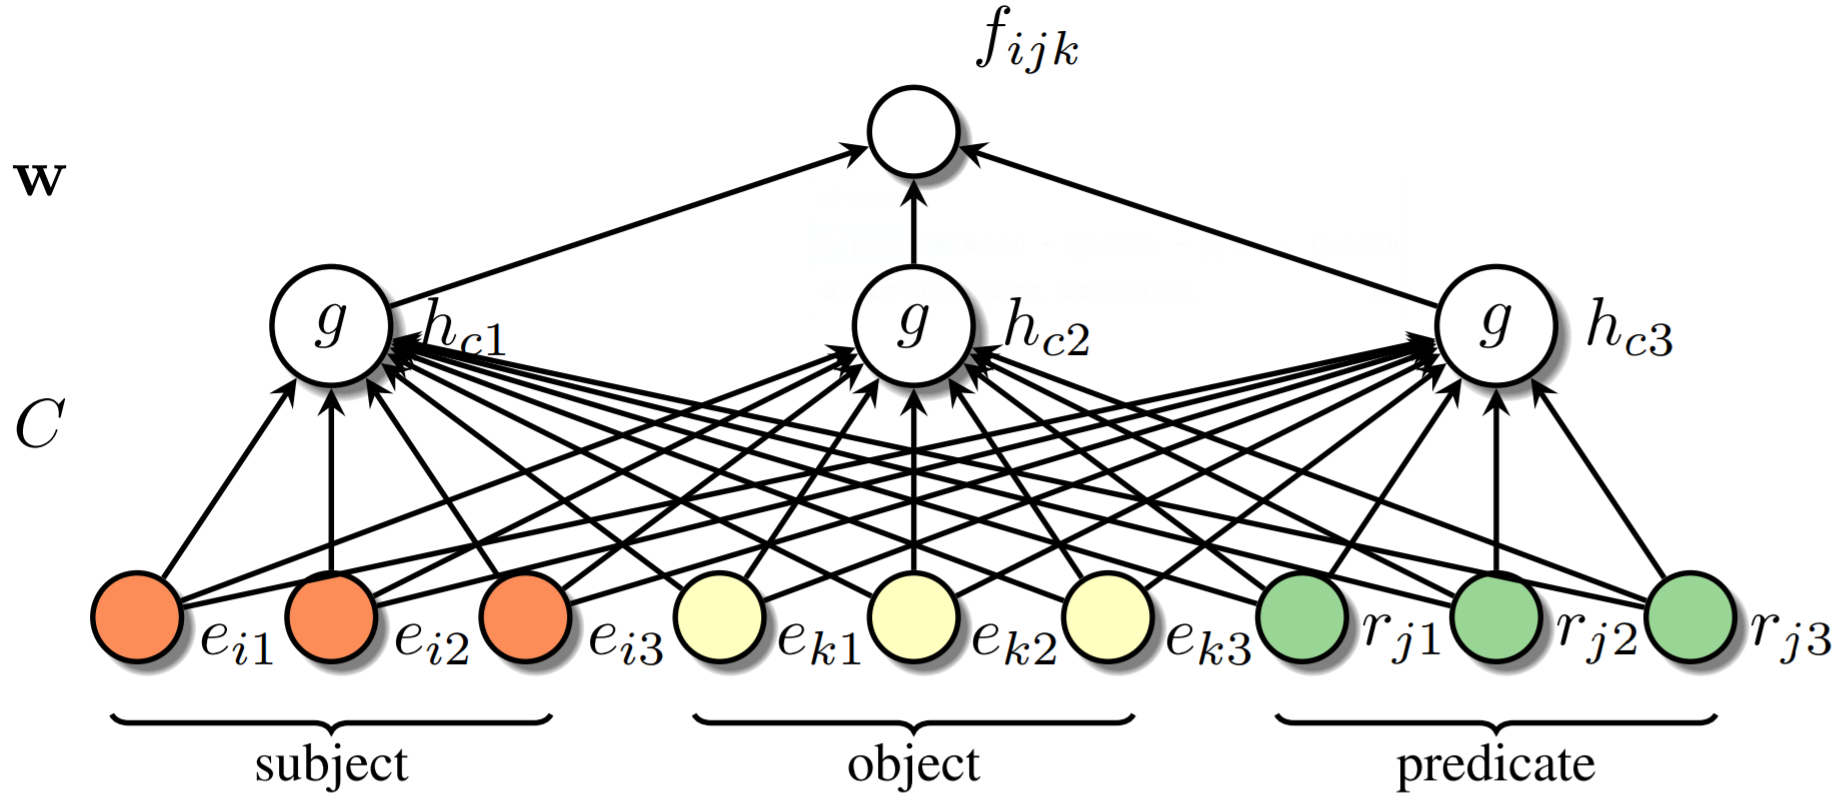
\includegraphics[width=0.48\columnwidth]{figure/rw/kbc-ermlp.png}}

  \vspace{1em}

  \subcaptionbox{TransE模型\label{fig:rw-kbe:c}}
    {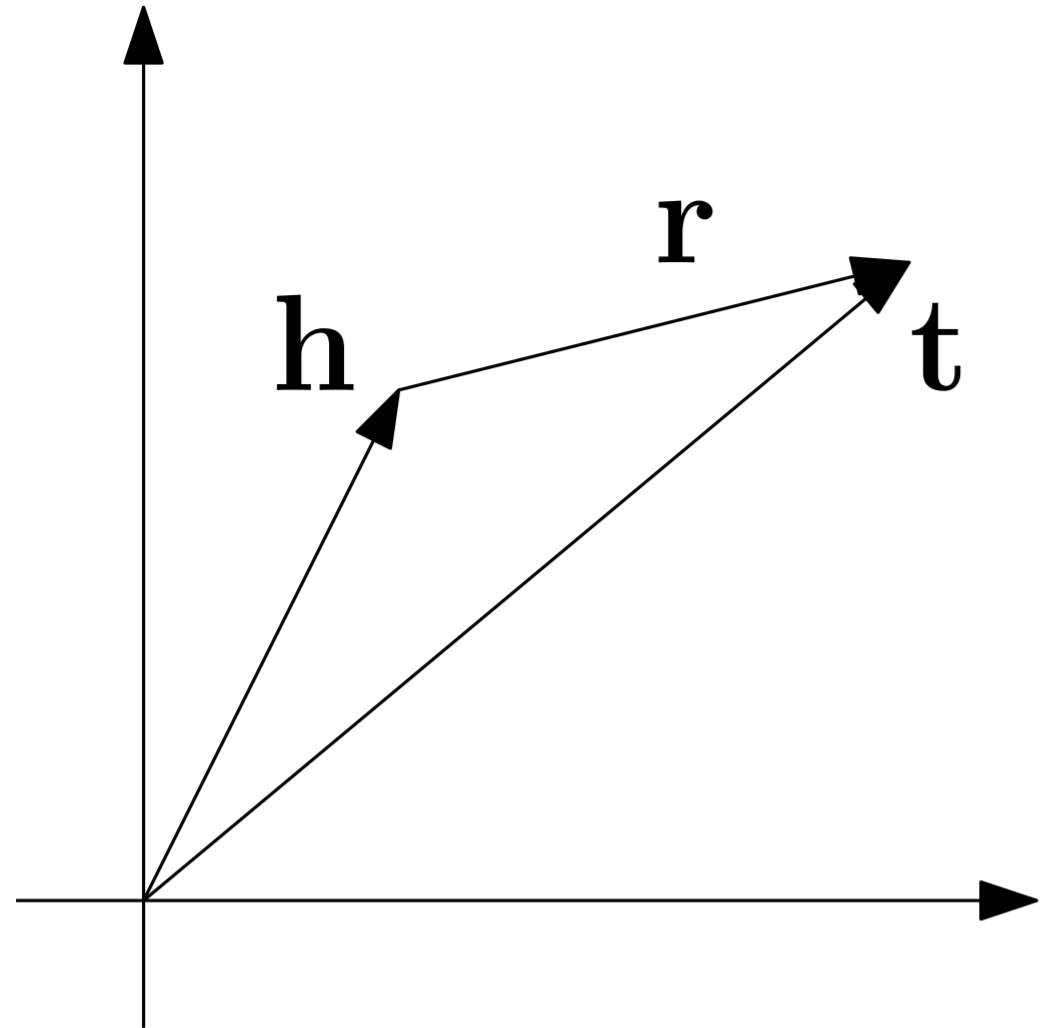
\includegraphics[width=0.30\columnwidth]{figure/rw/kbc-transe.png}}
  \hspace{4em}
  \subcaptionbox{TransH模型\label{fig:rw-kbe:d}}
    {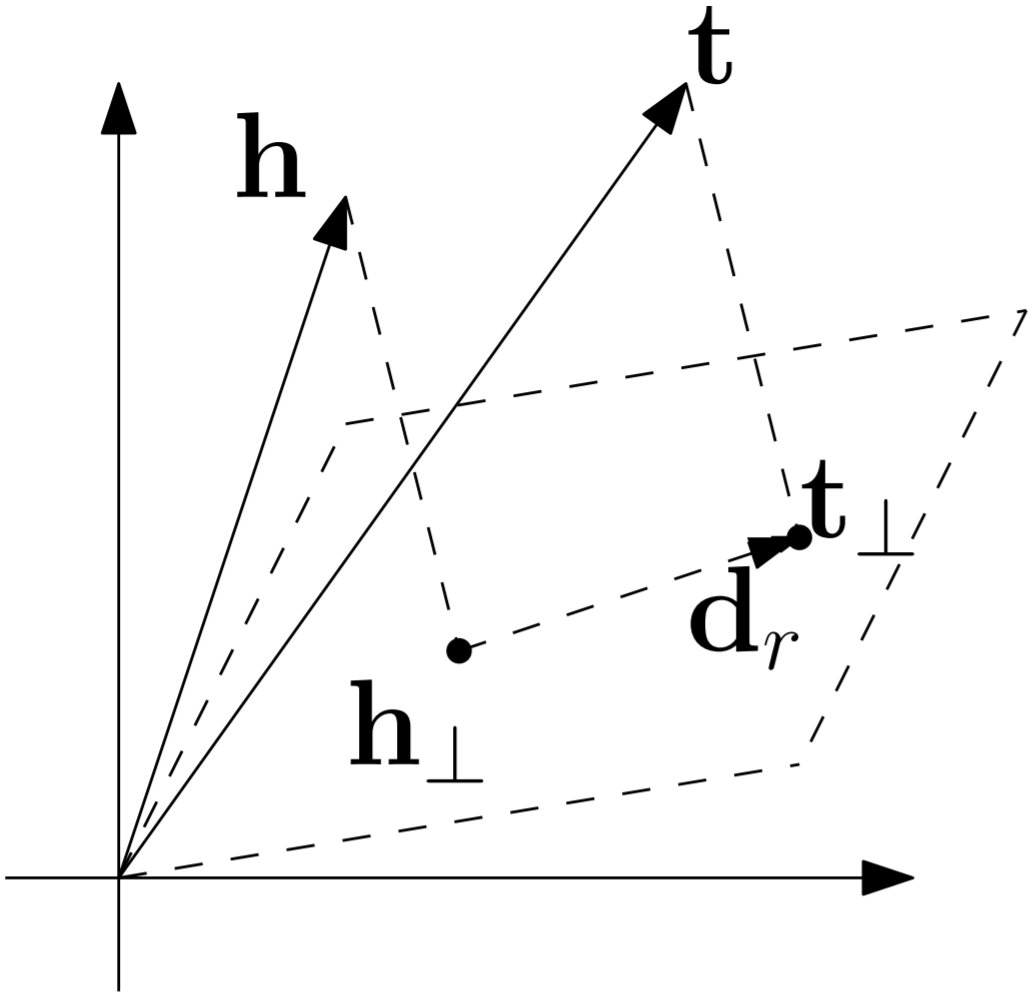
\includegraphics[width=0.30\columnwidth]{figure/rw/kbc-transh.png}}
  \bicaption{多种知识库向量模型示意图。\cite{nickel2016review,wang2014knowledge}}
            {Examples of knowledge base embedding models.}
  \label{fig:rw-kbe}
\end{figure}


由Nickel等人提出的RESCAL模型\cite{nickel2012factorizing}是一个基础的知识库向量模型,
模型对三元组($e_i$, $r_k$, $e_j$)置信分(简写为$S$)的定义,
基于主宾语实体特征表示的在不同维度间的两两交互:
\begin{equation}
S^{RESCAL} = \bm{e}_i^\top \bm{W}_k \bm{e}_j = \sum_{a=1}^d \sum_{b=1}^d w_{kab} e_{ia} e_{jb},
\end{equation}
\noindent
其中$\bm{e}_i$和$\bm{e}_j$为对应实体向量,维度为$d$。$\bm{W}_k \in \mathbb{R}^{d \times d}$
为谓词$r_k$的权重矩阵,其中$w_{kab}$体现了实体向量的第$i$和$j$维特征对于第$k$个谓词的交互重要性。
由于RESCAL使用矩阵连乘形式捕捉实体向量之间的交互,因此也被称为双线性模型。
如\figref{fig:rw-kbe:a}所示,RESCAL模型可表示为双层神经网络结构,
首先通过张量积(Tensor Product)构建实体对($e_i$, $e_j$)的组合特征,
再利用与特定谓词相关的参数$\bm{W}_k$作为权重,得到三元组最终的置信分。
RESCAL模型学习的实体特征表示能够捕捉不同实体间的语义相似性,
换言之,若两个实体可以通过相似的谓词连接至相似的其它实体,
那么它们的特征表达也更加相近。

%The shared entity representations
%in RESCAL capture also the similarity of entities in the
%relational domain, i.e., that entities are similar if they are
%connected to similar entities via similar relations [65].


RESCAL模型存在的一个问题在于参数量过大,每一个谓词对应参数量为$d \times d$,
对于拥有大量谓词的知识库而言,会带来可扩展性的问题。
一些后续研究对此进行了改进。
Socher等人以及Dong等人
分别提出了E-MLP\cite{socher2013reasoning}和ER-MLP模型\cite{dong2014knowledge}。
\figref{fig:rw-kbe:b}为ER-MLP的示意图,均由两层前向网络构成,
第一层用于学习三元组的组合特征表示,第二层则通过组合特征输出置信分。
E-MLP结构较为类似,故此处不专门画图。
两个模型的置信分计算如下:
\begin{equation}
\begin{aligned}
& S^{E-MLP} = \bm{w}_k^\top \bm{g}(\bm{C}_k [\bm{e}_i; \bm{e}_j]), \\
& S^{ER-MLP} = \bm{w}^\top \bm{g}(\bm{C} [\bm{e}_i; \bm{e}_j; \bm{r}_k]),
\end{aligned}
\end{equation}
\noindent
其中,$g$为非线性激活函数。
对比RESCAL模型,E-MLP的最大不同在于可以通过调整矩阵$\bm{C}_k$来学习实体间不同维度特征的交互,
从而优化实体对($e_i$, $e_j$)的组合特征表示,并大幅度减少参数数量。
E-MLP模型中,不同的谓词依然对应不同的参数,而ER-MLP模型将谓词也映射为向量表示,
与两实体共同作为第一层的输入,因此模型的参数$\bm{C}$与$\bm{w}$均与特定谓词无关。
两个模型依然能够让语义相似的实体映射至连续空间的相近位置。

Nickel等人提出了HOLE模型\cite{nickel2015holographic},
该模型利用循环相关运算(Circular Correlation)巧妙地代替了RESCAL中的张量积操作:
\begin{equation}
S^{HOLE} = \bm{w}_k^\top (\bm{e}_i \star \bm{e}_j) = \sum_{a=1}^d \sum_{b=0}^{d-1} w_{ka} e_{ia} e_{j,(a+b) \% d},
\end{equation}
\noindent
可以从公式中看出,循环相关运算等同于将张量积的结果进行了分组,模型通过对实体特征表示的学习,
让具有相似语义的特征交互归为同一组,共享同一个权重。
因此HOLE的优势在于将RESCAL中的二维矩阵参数降低至一维,同时尽可能保留了特征交互的表示能力,
并且在实验中效果优于RESCAL和ER-MLP模型。

此外,Socher等人还提出了较复杂的神经张量网络(Neural Tensor Networks,NTN)模型\cite{socher2013reasoning},
可以看做是RESCAL和E-MLP的组合体,对实体对($e_i$, $e_j$)构建的组合特征表达同时包括双线性和前向网络特征,
但模型参数量也因此更加庞大,在小数据集上更容易出现过拟合。



%1+3+1段
另一类 知识库向量模型   是以TransE为典型的 被称作 隐距离模型。
相比 RESCAL等模型 依照神经网络构建的置信分函数,
隐距离模型对置信分的计算则与距离度量直接相关。
这与\secref{sec:rw-linking-cle}介绍的跨语言词向量训练有着相似之处,
源语言词向量经过转换后,与翻译后的词向量尽可能相近。
而对于知识库向量模型,由于三元组中还有谓词的存在,
因此模型训练的实质,是学习主宾语实体向量在特定谓词下的变换方式,
对变换之后的向量表示进行距离度量,距离越近,则置信分越高。
为了和相关工作统一,此处用($h$, $r$, $t$)表示一个事实三元组。

Bordes等人提出的SE模型\cite{bordes2011learning}较为基本,
度量实体$h$和$t$经矩阵变换后的距离:
\begin{equation}
S^{SE} = -dist(\bm{A}_r^s \bm{h}, \bm{A}_r^o \bm{t}),
\end{equation}
\noindent
其中$dist(\cdot)$为距离度量函数,例如L1距离或欧氏距离。
谓词$r$对应两个参数矩阵,分别映射主语和宾语实体的向量表示至同一空间。
为了降低参数个数,Bordes等人提出了TransE模型\cite{bordes2013translating},
这也是后续很多改进模型的起点。
受到词向量之间代数运算的启发,
例如$queen \simeq king - man + woman$\cite{mikolov2013linguistic},
不同词之间的关系体现在了它们词向量的位置偏移中,
因此如\figref{fig:rw-kbe:c}所示,TransE模型共享了实体与谓词的特征表示,
利用在主语实体在同一空间中的平移变换,代替更加复杂的矩阵变换:
\begin{equation}
S^{TransE} = -dist(\bm{h} + \bm{r}, \bm{t} ).
\end{equation}

TransE模型设计简单、容易实现,并且具有训练速度快、可扩展性高等优点,
但是对于知识库中存在的一对多或多对一的谓词不友好,
例如固定主谓,TransE无法有效区分出多个匹配的宾语实体。
为此,TransH模型\cite{wang2014knowledge}尝试通过超平面投影来解决此问题,
公式定义如下:
\begin{equation}
  \bm{h}_\bot = \bm{h} - \bm{w}_r^\top \bm{h} \bm{w}_r, \ 
  \bm{t}_\bot = \bm{t} - \bm{w}_r^\top \bm{t} \bm{w}_r, \
  S^{TransH} = -dist(\bm{h}_\bot + \bm{d}_r, \bm{t}_\bot),
\end{equation}
\noindent
如\figref{fig:rw-kbe:d}所示,TransH首先把$h$和$t$的向量表示均投影到连续空间中,
谓词$r$对应的超平面上($\bm{w}_r$为单位法向量),
并学习谓词向量表示$\bm{d}_r$,在超平面上沿用TransE的度量。
因此,TransH具有更高的灵活度来应对一对多或多对一谓词,
同时依然保有TransE可扩展性高的特点。
TransR模型\cite{lin2015learning}同样尝试解决一对多谓词的问题,
类似于SE和TransE的组合体,利用投影矩阵$\bm{M}_r$将实体表示转移至新的空间后,
再进行基于平移的距离度量。
因此TransR模型中,实体和谓词的特征表达并不共享同一个语义空间,
这与TransE和TransH模型均不同:
\begin{equation}
S^{TransR} = -dist(\bm{M}_r \bm{h} + \bm{r}, \bm{M}_r \bm{t}).
\end{equation}

此外,还有其它TransE模型的改进工作,
包括体现距离度量在不同特征维度间差异的TransA\cite{xiao2015transa},
生成谓词多个表示以解决一对多问题的TransG\cite{xiao2016transg}等,这里不再展开讨论。

